\documentclass[tikz,border=10pt]{standalone}
\usepackage{tikz}
\usepackage{amsmath}
\usepackage{amssymb}

% TikZ libraries
\usetikzlibrary{calc}
\usetikzlibrary{positioning}

% Custom commands for mathematical notation
\newcommand{\cS}{\mathcal{S}}
\newcommand{\R}{\mathbb{R}}
\newcommand{\vx}{\boldsymbol{x}}
\newcommand{\norm}[1]{\left\|#1\right\|}
\newcommand{\dist}{\mathrm{dist}}
\newcommand{\set}[1]{\left\{#1\right\}}

\begin{document}
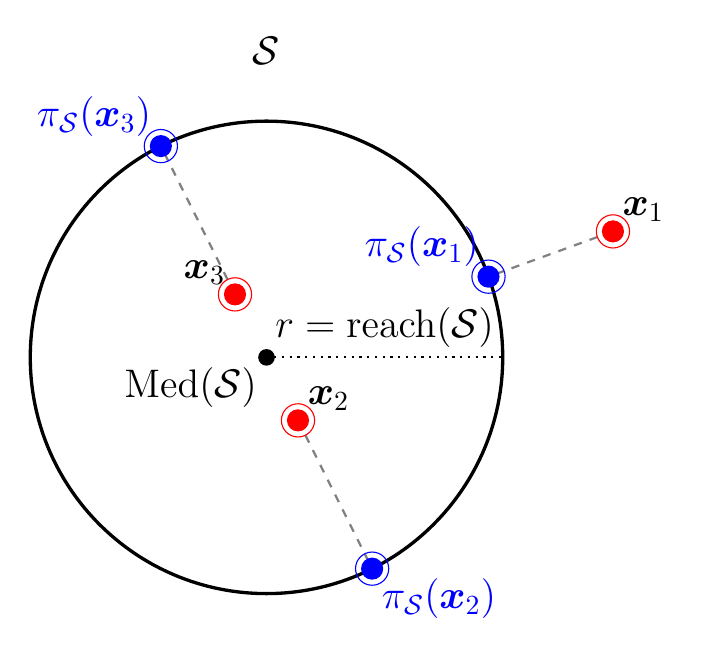
\begin{tikzpicture}[scale=2, font=\Large]
  % Define circle parameters
  \def\radius{1.5}
  \coordinate (center) at (0,0);

  % Draw the main circle S (black, thick)
  \draw[black, line width=1.2pt] (center) circle (\radius);

  % Define points
  \coordinate (p1) at (2.2, 0.8);     % Outside point
  \coordinate (p2) at (0.2, -0.4);    % Inside point 1 (antipodal to p3)
  \coordinate (p3) at (-0.2, 0.4);    % Inside point 2

  % Calculate projections onto circle
  % For outside point p1
  \pgfmathsetmacro{\angleone}{atan2(0.8, 2.2)}
  \pgfmathsetmacro{\projoneX}{\radius * cos(\angleone)}
  \pgfmathsetmacro{\projoneY}{\radius * sin(\angleone)}
  \coordinate (proj1) at (\projoneX, \projoneY);

  % For inside point p2
  \pgfmathsetmacro{\angletwo}{atan2(-0.4, 0.2)}
  \pgfmathsetmacro{\projtwoX}{\radius * cos(\angletwo)}
  \pgfmathsetmacro{\projtwoY}{\radius * sin(\angletwo)}
  \coordinate (proj2) at (\projtwoX, \projtwoY);

  % For inside point p3
  \pgfmathsetmacro{\anglethree}{atan2(0.4, -0.2)}
  \pgfmathsetmacro{\projthreeX}{\radius * cos(\anglethree)}
  \pgfmathsetmacro{\projthreeY}{\radius * sin(\anglethree)}
  \coordinate (proj3) at (\projthreeX, \projthreeY);

  % Draw projection lines (dashed)
  \draw[dashed, gray, line width=0.8pt] (p1) -- (proj1);
  \draw[dashed, gray, line width=0.8pt] (p2) -- (proj2);
  \draw[dashed, gray, line width=0.8pt] (p3) -- (proj3);

  % Draw medial axis (center point) - special styling
  \fill[black] (center) circle (1.5pt);
  \node[below left] at (center) {$\mathrm{Med}(\mathcal{S})$};

  % Draw points
  \fill[red] (p1) circle (2pt);
  \fill[red] (p2) circle (2pt);
  \fill[red] (p3) circle (2pt);

  % Draw projected points
  \fill[blue] (proj1) circle (2pt);
  \fill[blue] (proj2) circle (2pt);
  \fill[blue] (proj3) circle (2pt);

  % Labels for points
  \node[above right] at (p1) {$\boldsymbol{x}_1$};
  \node[above right] at (p2) {$\boldsymbol{x}_2$};
  \node[above left] at (p3) {$\boldsymbol{x}_3$};

  % Labels for projected points
  \node[above left, blue] at (proj1) {$\pi_{\mathcal{S}}(\boldsymbol{x}_1)$};
  \node[below right, blue] at (proj2) {$\pi_{\mathcal{S}}(\boldsymbol{x}_2)$};
  \node[above left, blue] at (proj3) {$\pi_{\mathcal{S}}(\boldsymbol{x}_3)$};

  % Draw radius line to illustrate reach
  \draw[dotted, thick] (center) -- (1.5, 0);
  \node[above] at (0.75, 0) {$r = \mathrm{reach}(\mathcal{S})$};

  % Label the set
  \node[above] at (0, \radius + 0.3) {$\mathcal{S}$};

  % Add small circles around points for emphasis
  \draw[red, thin] (p1) circle (3pt);
  \draw[red, thin] (p2) circle (3pt);
  \draw[red, thin] (p3) circle (3pt);

  \draw[blue, thin] (proj1) circle (3pt);
  \draw[blue, thin] (proj2) circle (3pt);
  \draw[blue, thin] (proj3) circle (3pt);

\end{tikzpicture}
\end{document}
